\section{Развертывание сайта}
Их схемы развертывания (рис. \ref{ris:deployment_sait}) видно что развертывание - это
многоэтапный процесс в котором важна последовательность этапов. Так же важно учитывать что приложение
считается обноленным только в случае если все этапы выполнены успешно. В случае
неуспешного выполения хотя бы одного из этапов необходимо обратить все
изменения. Исходя из анных фактов вытекает важно требования для системы
развертывания - транзакционность, т.е. любое изменение должно быть обратимо.

\begin{figure}[h!]
\center{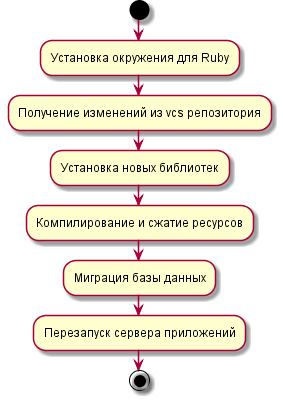
\includegraphics[width=0.5\linewidth]{deployment_sait.eps}}
\caption{Схема развертывания Ruby On Rails сайта}
\label{ris:deployment_sait}
\end{figure}

Для развертывания и обновления сайта на рабочем сервере существует библиотека
Capistrano. Данная библиотека позволяет настроить полностью контролируемый
процесс развертывания сайта.

Основные преимущества от использования данной библиотеки:
\begin{enumerate}
  \item поддержка транзакций и возможность обратить все изменения;
  \item гибкая настройка процесса за счет возможности выполнять любой удаленный
  \item код на сервере; 
  \item поддержка протокола ssh - необходимо для обеспечения безопасности; 
  \item интеграция с Ruby On Rails;
  \item развертывание на несколько серверов одновременно;
  \item установка окружения ruby.
\end{enumerate}

На данном этапе разработки библиотека не используется, так как нет необходимости
разворачивать приложение на рабочем сервере.

Рассмотрим инструкцию для запуска сайта в режиме разработчика.

В качестве операционой системы можно использовать любой UNIX-like дистрибутив.

Для начала нужно уставновить окружение для работы ruby, установку лучше всего
производить через rvm. Для работы проекта требуется ruby версии 1.9.3.

Далее необходимо установить базу данных Postgresql и создать пользователя в базе
данных с правами на создание баз данных. В конфигурационно файле
config/database.yml в секции development нужно выставить соответствующие логин и
пароль ждя подключения к базе данных.

Следующим шагом создадим непосредственно базу данных с помощью команды rake
db:create. База данных создана, но в ней нет необходимых таблиц. Чтобы добавить
таблицы в базу данных выполним rake db:migrate.

Для работы сайта создадим набор тестовых данных с помощью команды rake db:seed.

Запустим Websocket сервер с помощью команды rake wsserver.

Теперь можно запускать непосредственно сайт - rails s. После чего сайт будет
доступен по адресу \url{http://localhost:3000}.